\chapter{Tau Identification Studies}
\label{chap:TauIDStudies}

The CMS Collaboration has groups of persons specialized in each 
object reconstruction, in the case of the tau reconstruction is called 
the TAU Particle Object Group (TAUPOG). The TAUPOG suggest criteria
for the tau identification, such as the WP for each discriminator. The 
\tauh~identification criteria recommended by the TAUPOG are different 
from those used in this analysis. However, a comparison between any 
recommended \\
 The selection of the working points for the discriminators is 
 based on the sensitivity reached in the \Zprimetotauh~channel
 as well as the consistency with the \tauh~identification criteria
 used in the others di-tau channels. 



\section{Number of prongs Study}
\label{Results:TauID-nprongs}

 \begin{tiny} 
 \begin{table}[ht] 
 \centering{ 
 \begin{tabular}{ | l | r | r |} \hline \hline 
 \multicolumn{3}{|c|}{\textcolor{red}{OVERALL YIELDS} } \\ \hline 
 & \textcolor{red}{1 or 3 prongs} &  \textcolor{red}{1 or 2 or 3 prongs}  \\ \hline \hline 
 DY         & 131.61   $\pm$   8.64 & 151.98   $\pm$   9.09 \\ \hline 
 WJets      & 41.91   $\pm$   5.17 & 65.18   $\pm$   8.41 \\ \hline 
 DiBoson    & 3.73   $\pm$   1.07 & 4.71   $\pm$   1.21 \\ \hline 
 TTbar      & 4.39   $\pm$   1.23 & 5.72   $\pm$   1.41 \\ \hline 
 QCD        & 382.67   $\pm$   24.84 & 753.06   $\pm$   34.33 \\ \hline 
 TOTAL BKG  & 564.30   $\pm$   26.86 & 980.65   $\pm$   36.54 \\ \hline 
 \Zprime~(3 \TeV)   & 1.91   $\pm$   0.02 & 2.35   $\pm$   0.02 \\ \hline  \hline 
 \end{tabular} 
 } 
 \end{table} 
 \end{tiny} 
 \vspace{-0.5cm} 
 \begin{tiny} 
 \begin{table}[ht] 
 \centering{ 
 \begin{tabular}{ | l | r | r |} \hline \hline 
 \multicolumn{3}{|c|}{\textcolor{red}{YIELD FOR $m\left(\tau_{1},\tau_{2}, \not\!\!E_{T}  \right)$ ABOVE 600~\GeV }} \\ \hline 
 & \textcolor{red}{1 or 3 prongs} &  \textcolor{red}{1 or 2 or 3 prongs}  \\ \hline \hline 
 $Data^{C}$            & 12.00   $\pm$   3.46 & 31.00   $\pm$   5.57 \\ \hline 
 $nonQCD^{C}$          & 1.80   $\pm$   0.65 & 4.36   $\pm$   0.96 \\ \hline 
 $Data^{C}-nonQCD^{C}$ & 10.20   $\pm$   3.52 & 26.64   $\pm$   5.65 \\ \hline 
 QCD                   & 13.67   $\pm$   4.72 & 35.70   $\pm$   7.57 \\ \hline 
 DY                    & 11.54   $\pm$   0.97 & 15.55   $\pm$   1.16 \\ \hline 
 W+Jets                & 2.02   $\pm$   0.80 & 2.88   $\pm$   0.97 \\ \hline 
 \textcolor{red}{TOTAL BKG}   & \textcolor{red}{28.63   $\pm$   4.94}  & \textcolor{red}{56.84   $\pm$   7.78} \\ \hline 
 \textcolor{blue}{\Zprime~(3 \TeV)}   & \textcolor{blue}{1.86   $\pm$   0.02} & \textcolor{blue}{2.30   $\pm$   0.02} \\ \hline 
 \textbf{\textcolor{green}{SIGNIFICANCE}} & \textcolor{green}{ 0.34} & \textcolor{green}{ 0.30} \\ \hline  \hline
 \end{tabular} 
 } 
 \end{table} 
 \end{tiny} 


\begin{figure}[ht]
\begin{center}
\captionsetup[subfloat]{farskip=0pt,captionskip=0.0cm,labelformat=empty}
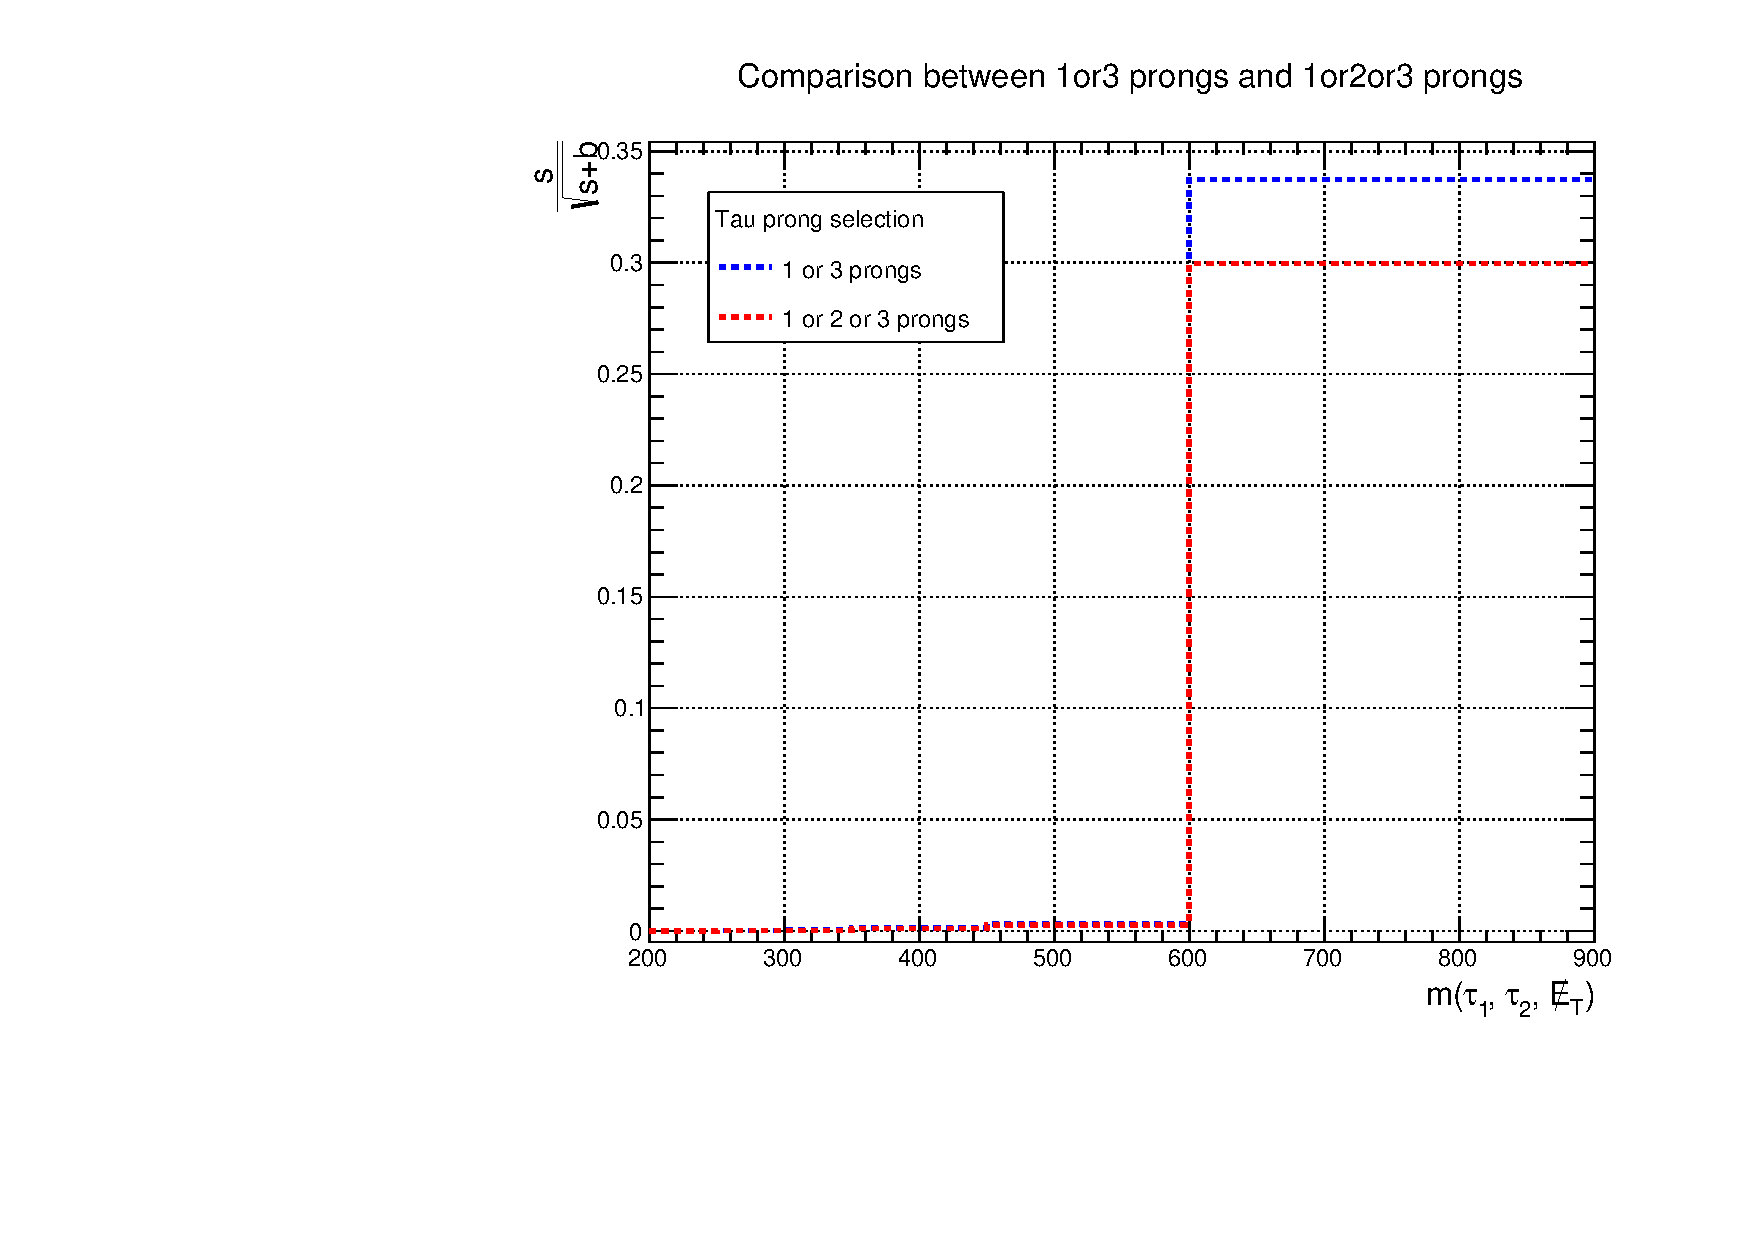
\includegraphics[clip,width=0.5\textwidth]{figuras/AppendiceB/2prongs/prongsComparison.pdf}
\end{center}
\end{figure}

\section{MVA-based Isolation Discriminator Study}
\label{Results:TauID-isoDicr}

\begin{figure}[ht]
\begin{center}
\captionsetup[subfloat]{farskip=0pt,captionskip=0.0cm,labelformat=empty}
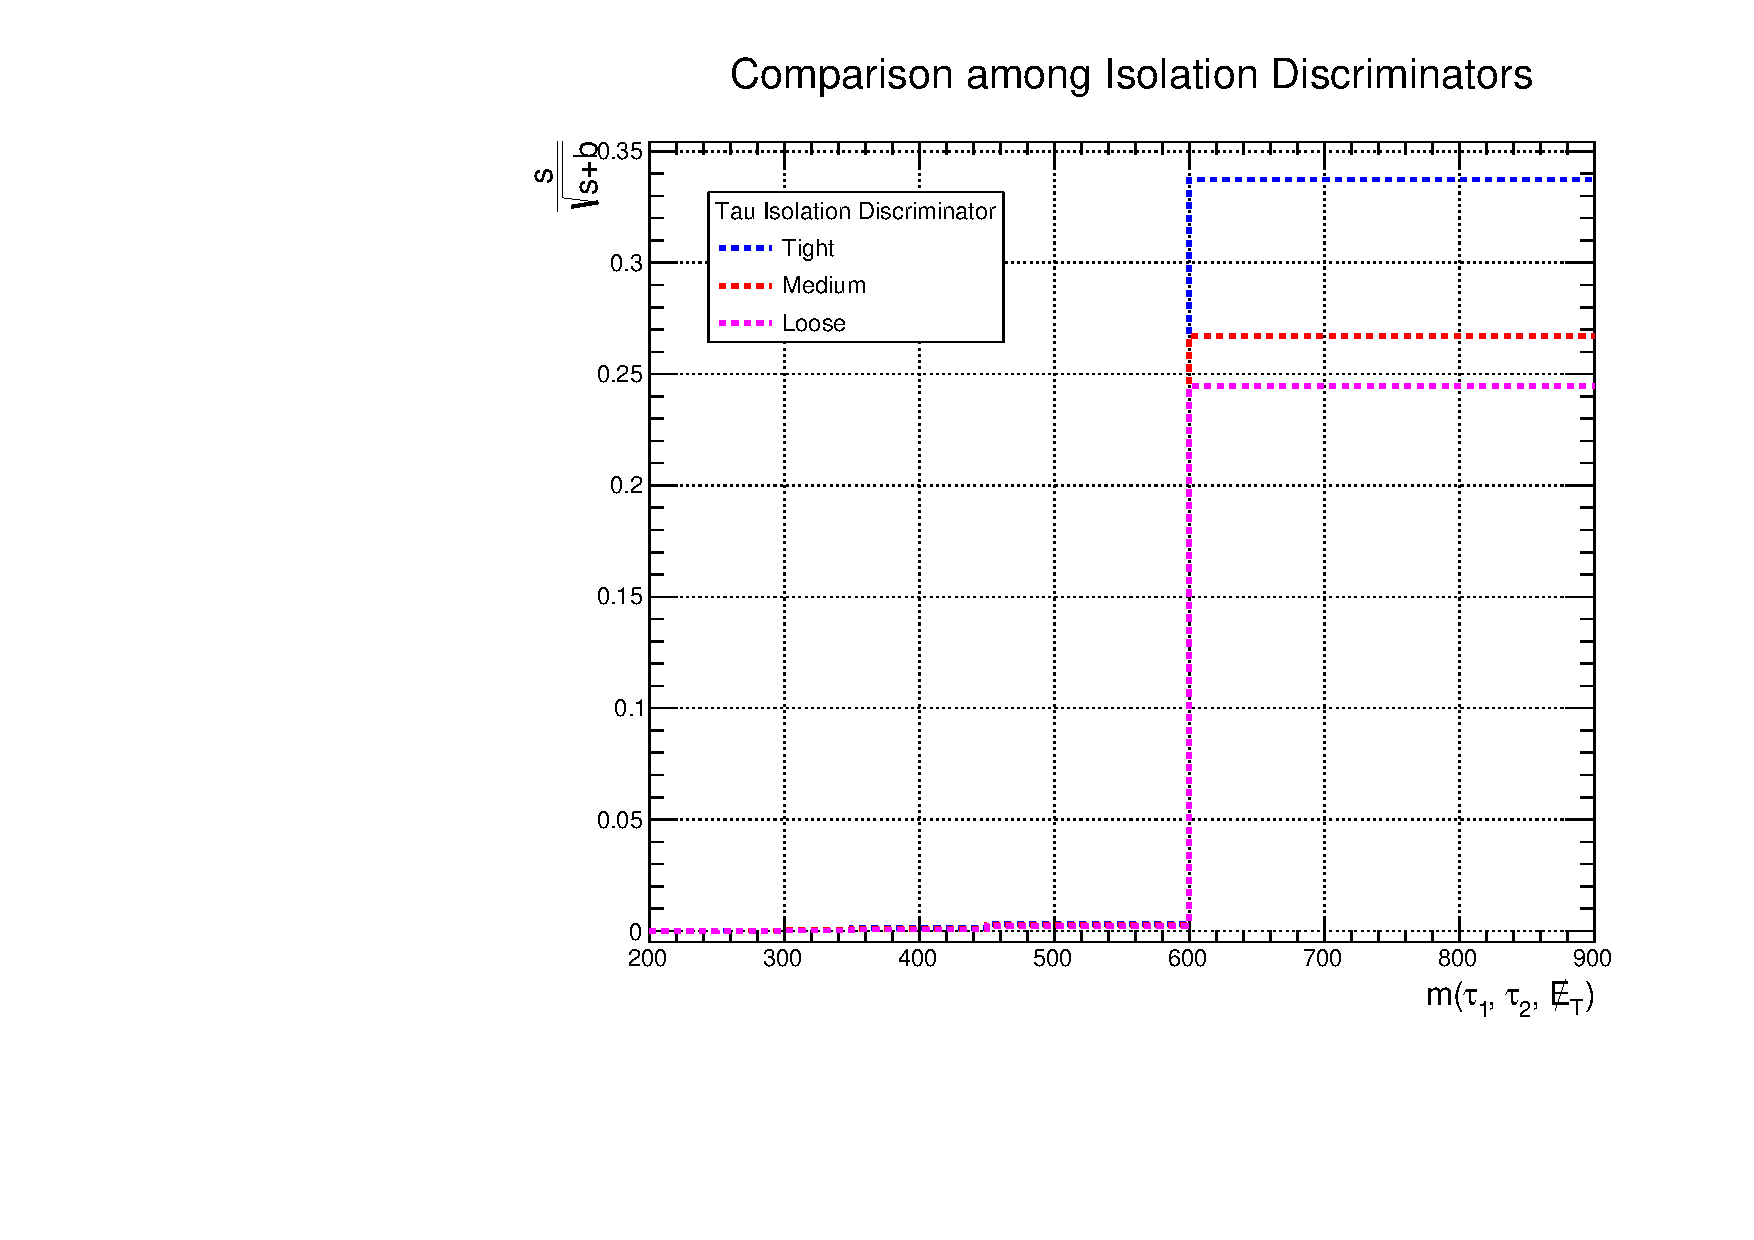
\includegraphics[clip,width=0.5\textwidth]{figuras/AppendiceB/IsoDiscr/IsoDiscrComparison.pdf}
\end{center}
\end{figure}

\section{MVA-based against Electron Discriminator Study}
\label{Results:TauID-isoDicr}

 \begin{tiny} 
 \begin{table}[ht] 
 \centering{ 
 \begin{tabular}{ | l | r | r |} \hline \hline 
 \multicolumn{3}{|c|}{\textcolor{red}{OVERALL YIELDS} } \\ \hline 
 & \textcolor{red}{Loose} &  \textcolor{red}{VeryLoose}  \\ \hline \hline 
 DY         & 131.61   $\pm$   8.64 & 142.77   $\pm$   9.09 \\ \hline 
 WJets      & 41.91   $\pm$   5.17 & 47.52   $\pm$   5.52 \\ \hline 
 DiBoson    & 3.73   $\pm$   1.07 & 3.76   $\pm$   1.07 \\ \hline 
 TTbar      & 4.39   $\pm$   1.23 & 5.40   $\pm$   1.37 \\ \hline 
 QCD        & 382.67   $\pm$   24.84 & 400.68   $\pm$   25.35 \\ \hline 
 TOTAL BKG  & 564.30   $\pm$   26.86 & 600.13   $\pm$   27.55 \\ \hline 
 \Zprime~(3 \TeV)   & 1.91   $\pm$   0.02 & 2.19   $\pm$   0.02 \\ \hline  \hline 
 \end{tabular} 
 } 
 \end{table} 
 \end{tiny} 
 \vspace{-0.5cm} 
 \begin{tiny} 
 \begin{table}[ht] 
 \centering{ 
 \begin{tabular}{ | l | r | r |} \hline \hline 
 \multicolumn{3}{|c|}{\textcolor{red}{YIELD FOR $m\left(\tau_{1},\tau_{2}, \not\!\!E_{T}  \right)$ ABOVE 600~\GeV }} \\ \hline 
 & \textcolor{red}{Loose} &  \textcolor{red}{VeryLoose}  \\ \hline \hline 
 $Data^{C}$            & 12.00   $\pm$   3.46 & 14.00   $\pm$   3.74 \\ \hline 
 $nonQCD^{C}$          & 1.80   $\pm$   0.65 & 2.07   $\pm$   0.67 \\ \hline 
 $Data^{C}-nonQCD^{C}$ & 10.20   $\pm$   3.52 & 11.93   $\pm$   3.80 \\ \hline 
 QCD                   & 13.67   $\pm$   4.72 & 15.99   $\pm$   5.09 \\ \hline 
 DY                    & 11.54   $\pm$   0.97 & 12.52   $\pm$   1.03 \\ \hline 
 W+Jets                & 2.02   $\pm$   0.80 & 3.31   $\pm$   1.09 \\ \hline 
 \textcolor{red}{TOTAL BKG}   & \textcolor{red}{28.63   $\pm$   4.94}  & \textcolor{red}{33.21   $\pm$   5.36} \\ \hline 
 \textcolor{blue}{\Zprime~(3 \TeV)}   & \textcolor{blue}{1.86   $\pm$   0.02} & \textcolor{blue}{2.15   $\pm$   0.02} \\ \hline 
 \textbf{\textcolor{green}{SIGNIFICANCE}} & \textcolor{green}{ 0.34} & \textcolor{green}{ 0.36} \\ \hline  \hline
 \end{tabular} 
 } 
 \end{table} 
 \end{tiny} 
 
\begin{figure}[ht]
\begin{center}
\captionsetup[subfloat]{farskip=0pt,captionskip=0.0cm,labelformat=empty}
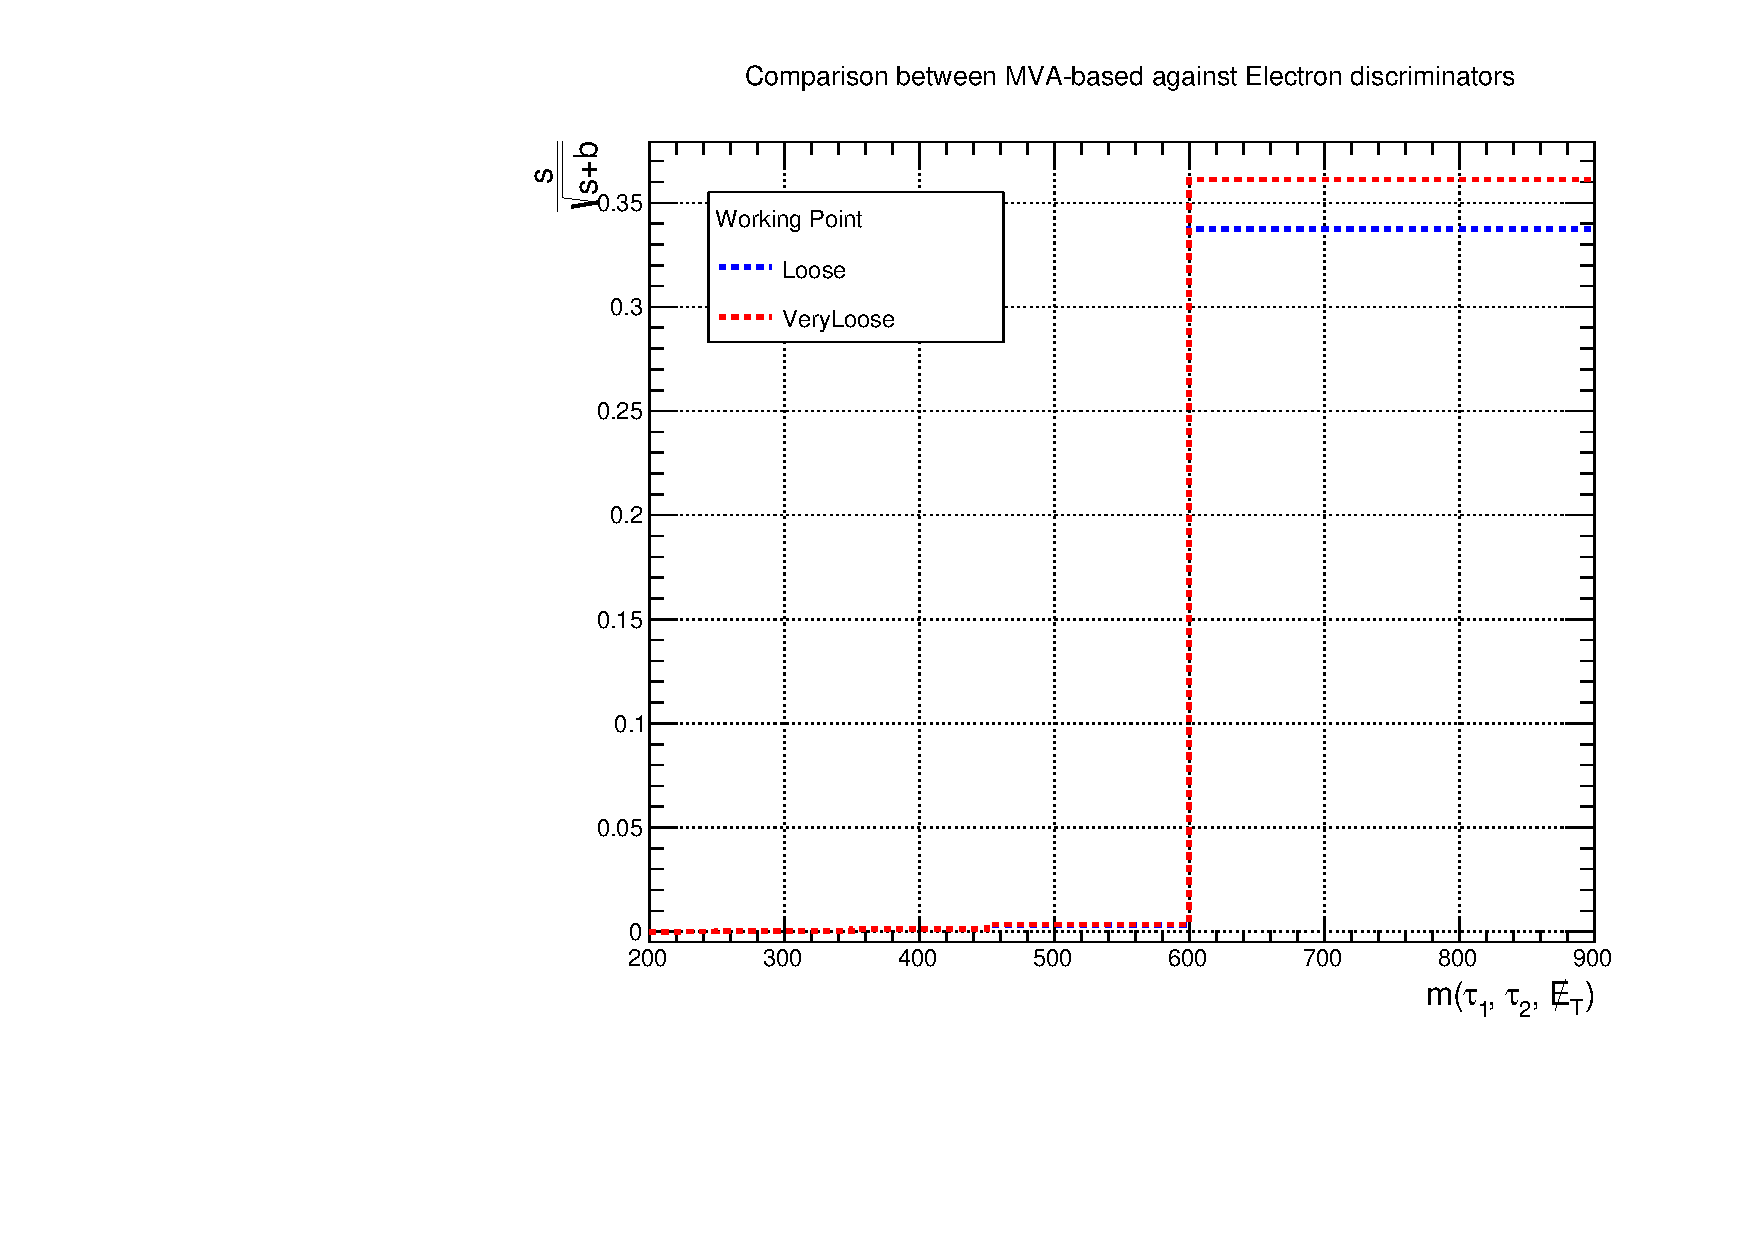
\includegraphics[clip,width=0.5\textwidth]{figuras/AppendiceB/againstElectronWP/againstElectron.pdf}
\end{center}
\end{figure}


\section{MVA-based against Muon Discriminator Study}
\label{Results:TauID-isoDicr}

  \begin{tiny} 
 \begin{table}[ht] 
 \centering{ 
 \begin{tabular}{ | l | r | r |} \hline \hline 
 \multicolumn{3}{|c|}{\textcolor{red}{OVERALL YIELDS} } \\ \hline 
 & \textcolor{red}{Tight} &  \textcolor{red}{Loose}  \\ \hline \hline 
 DY         & 131.61   $\pm$   8.64 & 132.84   $\pm$   8.67 \\ \hline 
 WJets      & 41.91   $\pm$   5.17 & 41.94   $\pm$   5.17 \\ \hline 
 DiBoson    & 3.73   $\pm$   1.07 & 3.73   $\pm$   1.07 \\ \hline 
 TTbar      & 4.39   $\pm$   1.23 & 4.39   $\pm$   1.23 \\ \hline 
 QCD        & 382.67   $\pm$   24.84 & 392.02   $\pm$   25.09 \\ \hline 
 TOTAL BKG  & 564.30   $\pm$   26.86 & 574.91   $\pm$   27.10 \\ \hline 
 \Zprime~(3 \TeV)   & 1.91   $\pm$   0.02 & 1.98   $\pm$   0.02 \\ \hline  \hline 
 \end{tabular} 
 } 
 \end{table} 
 \end{tiny} 
 \vspace{-0.5cm} 
 \begin{tiny} 
 \begin{table}[ht] 
 \centering{ 
 \begin{tabular}{ | l | r | r |} \hline \hline 
 \multicolumn{3}{|c|}{\textcolor{red}{YIELD FOR $m\left(\tau_{1},\tau_{2}, \not\!\!E_{T}  \right)$ ABOVE 600~\GeV }} \\ \hline 
 & \textcolor{red}{Tight} &  \textcolor{red}{Loose}  \\ \hline \hline 
 $Data^{C}$            & 12.00   $\pm$   3.46 & 12.00   $\pm$   3.46 \\ \hline 
 $nonQCD^{C}$          & 1.80   $\pm$   0.65 & 1.81   $\pm$   0.65 \\ \hline 
 $Data^{C}-nonQCD^{C}$ & 10.20   $\pm$   3.52 & 10.19   $\pm$   3.52 \\ \hline 
 QCD                   & 13.67   $\pm$   4.72 & 13.65   $\pm$   4.72 \\ \hline 
 DY                    & 11.54   $\pm$   0.97 & 11.86   $\pm$   0.99 \\ \hline 
 W+Jets                & 2.02   $\pm$   0.80 & 2.06   $\pm$   0.80 \\ \hline 
 \textcolor{red}{TOTAL BKG}   & \textcolor{red}{28.63   $\pm$   4.94}  & \textcolor{red}{28.96   $\pm$   4.94} \\ \hline 
 \textcolor{blue}{\Zprime~(3 \TeV)}   & \textcolor{blue}{1.86   $\pm$   0.02} & \textcolor{blue}{1.94   $\pm$   0.02} \\ \hline 
 \textbf{\textcolor{green}{SIGNIFICANCE}} & \textcolor{green}{ 0.34} & \textcolor{green}{ 0.35} \\ \hline  \hline
 \end{tabular} 
 } 
 \end{table} 
 \end{tiny} 
 
 
\begin{figure}[ht]
\begin{center}
\captionsetup[subfloat]{farskip=0pt,captionskip=0.0cm,labelformat=empty}
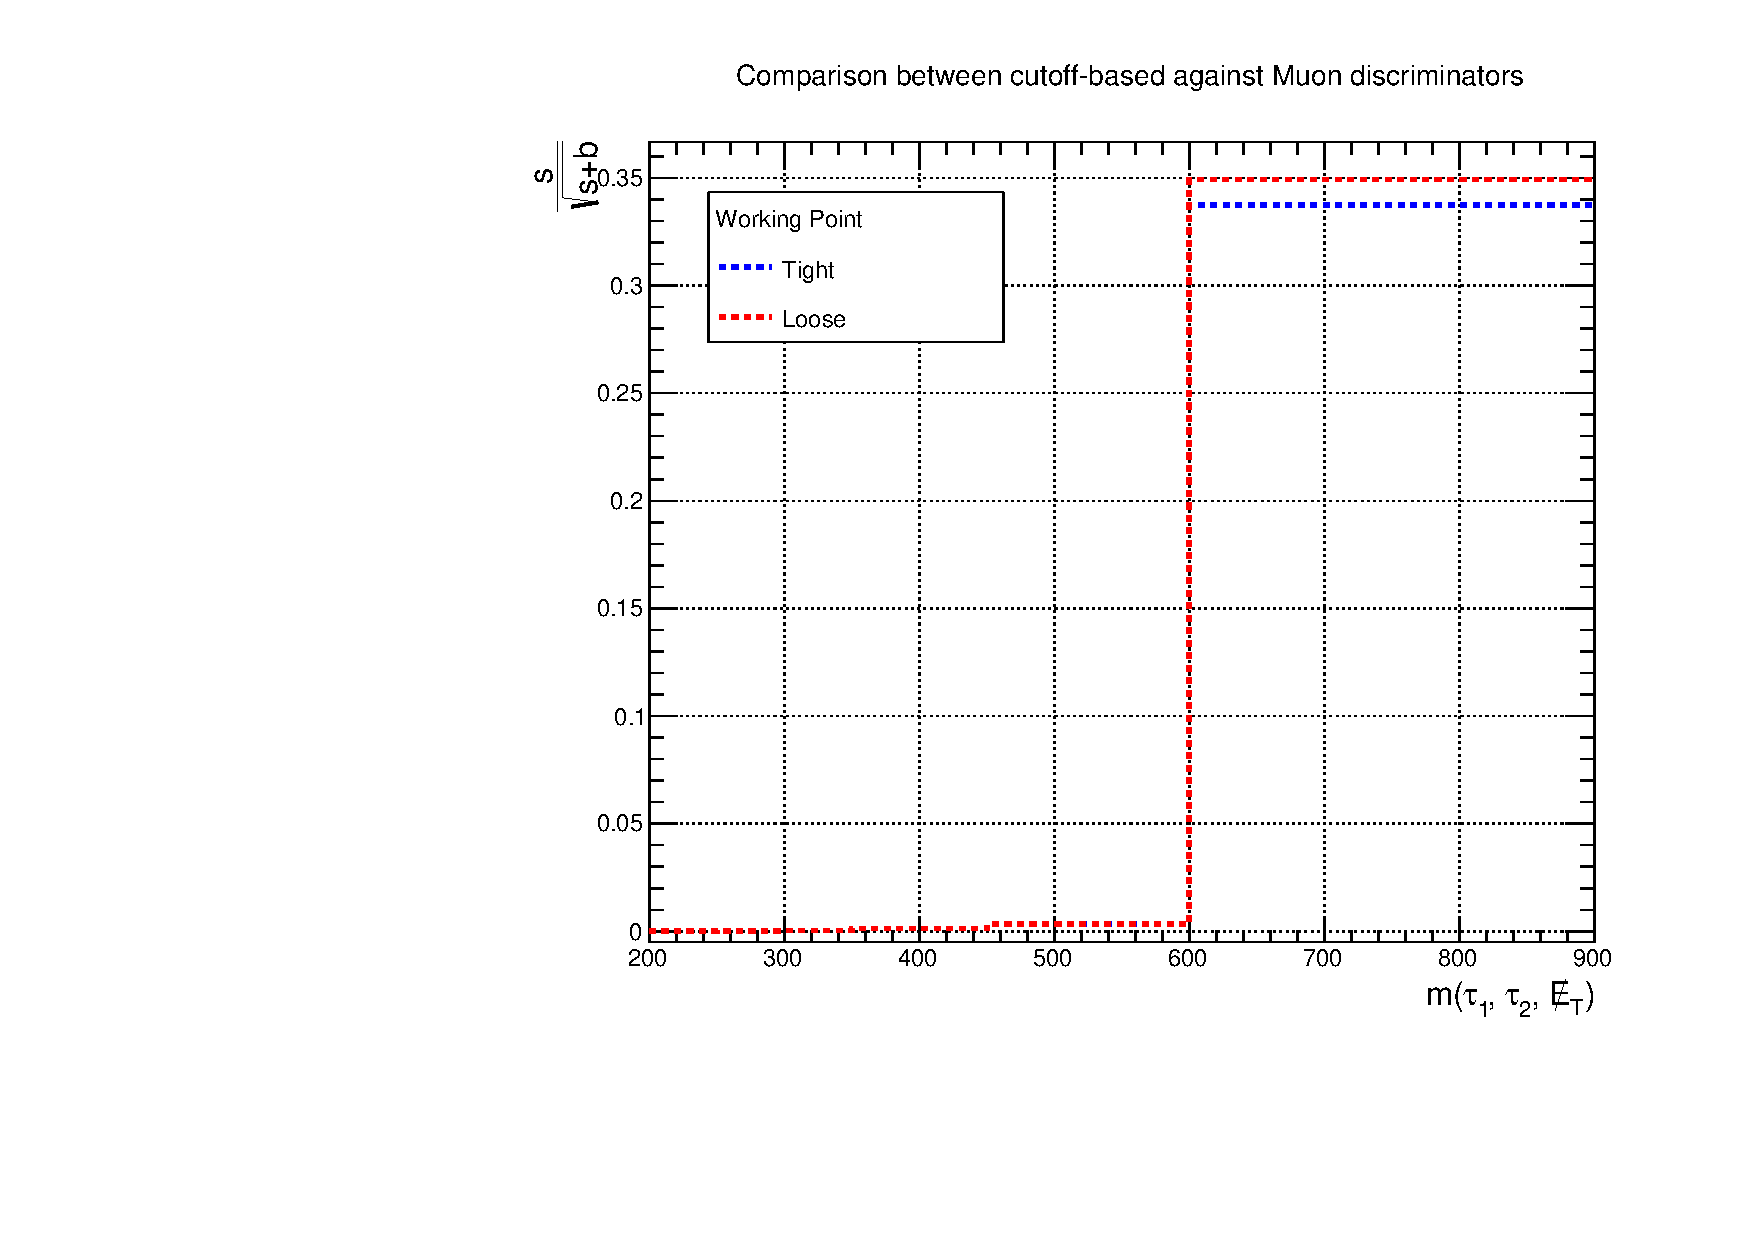
\includegraphics[clip,width=0.5\textwidth]{figuras/AppendiceB/againstMuonWP/againstMuon.pdf}
\end{center}
\end{figure}